\documentclass[11pt, oneside]{article}   	% use "amsart" instead of "article" for AMSLaTeX format
\usepackage{geometry}                		% See geometry.pdf to learn the layout options. There are lots.
\geometry{letterpaper}                   		% ... or a4paper or a5paper or ... 
%\geometry{landscape}                		% Activate for for rotated page geometry
%\usepackage[parfill]{parskip}    		% Activate to begin paragraphs with an empty line rather than an indent
\usepackage{graphicx}				% Use pdf, png, jpg, or eps§ with pdflatex; use eps in DVI mode
								% TeX will automatically convert eps --> pdf in pdflatex		
\usepackage{amssymb}

\title{}
\author{}
\date{}							% Activate to display a given date or no date

\begin{document}

\section*{Supplementary Information for ``Does Media Coverage Drive Public Support for UKIP or Does Public Support
for UKIP Drive Media Coverage?"}

\begin{figure}[htbp]
\centering
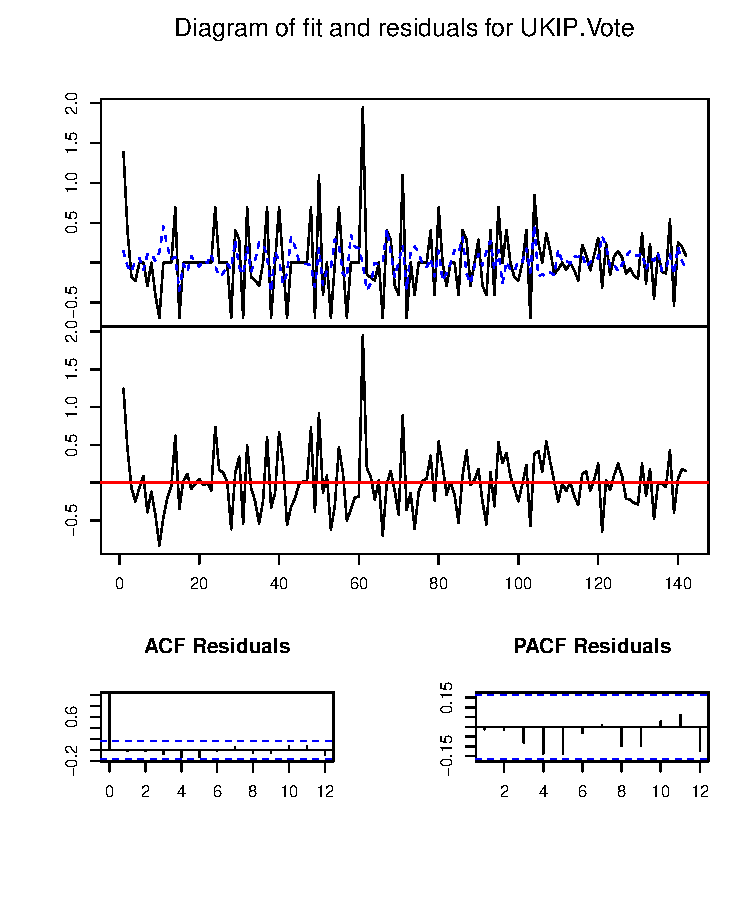
\includegraphics[scale=.9]{ukip_media_files/var-plot-support.pdf}
\caption{VAR Diagnostics for Support}
\end{figure}

\begin{figure}[htbp]
\centering
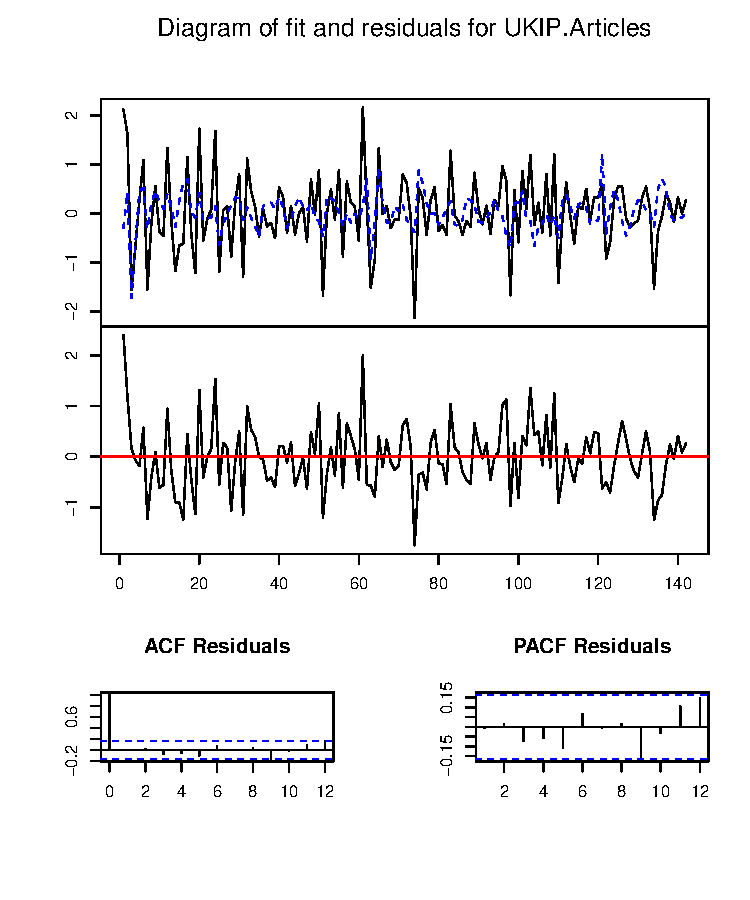
\includegraphics{ukip_media_files/var-plot-articles.pdf}
\caption{VAR Diagnostics for Articles}
\end{figure}

\pagebreak

\begin{figure}[htbp]
\centering
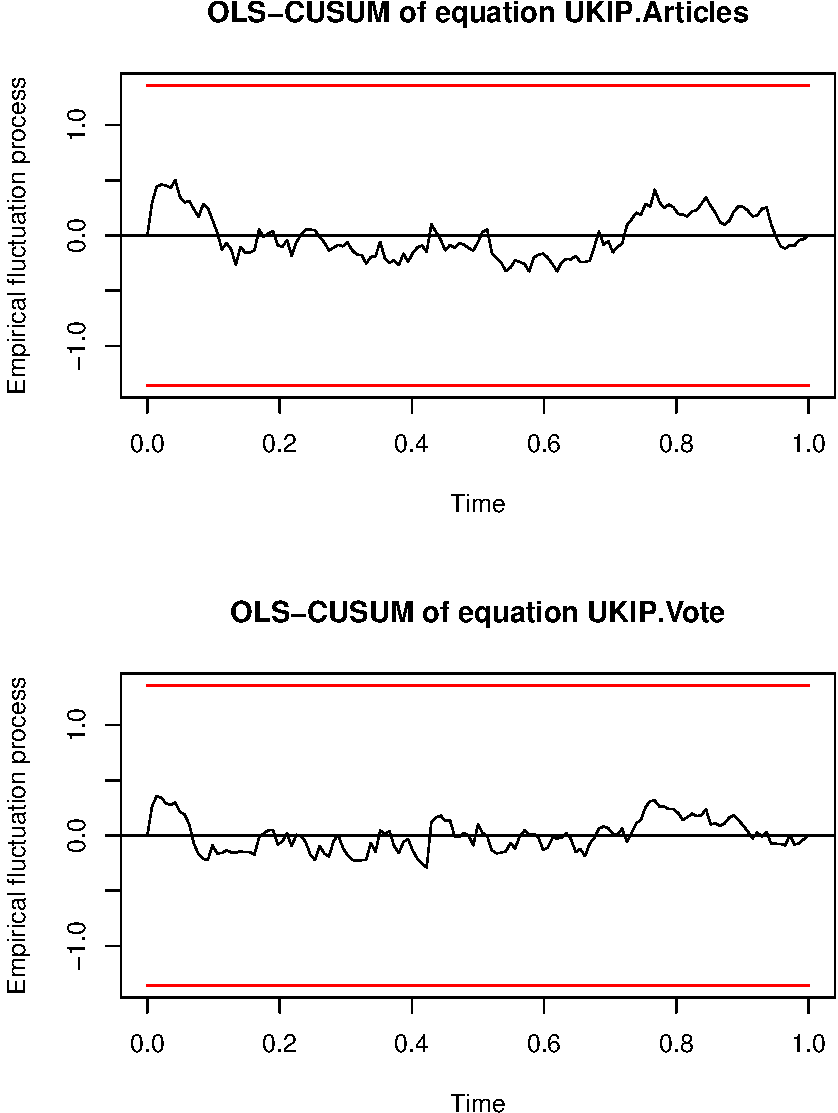
\includegraphics{ukip_media_files/figure-latex/stability-check-vote-1.pdf}
\caption{Checking temporal stability of VAR model with cumulative sums
of residuals}
\end{figure}

\newpage

\subsection*{Breusch-Godrey Test of serially correlated errors for VAR
model}\label{breusch-godrey-test-of-serially-correlated-errors-for-var-model}

\begin{verbatim}
## 
##  Breusch-Godfrey LM test
## 
## data:  Residuals of VAR object varmodel
## Chi-squared = 20, df = 20, p-value = 0.2
\end{verbatim}

\subsection*{Multivariate ARCH-LM test for heteroskedasticity in Var
model}\label{multivariate-arch-lm-test-for-heteroskedasticity-in-var-model}

\begin{verbatim}
## 
##  ARCH (multivariate)
## 
## data:  Residuals of VAR object varmodel
## Chi-squared = 40, df = 40, p-value = 0.8
\end{verbatim}

\newpage

\begin{figure}[htbp]
\centering
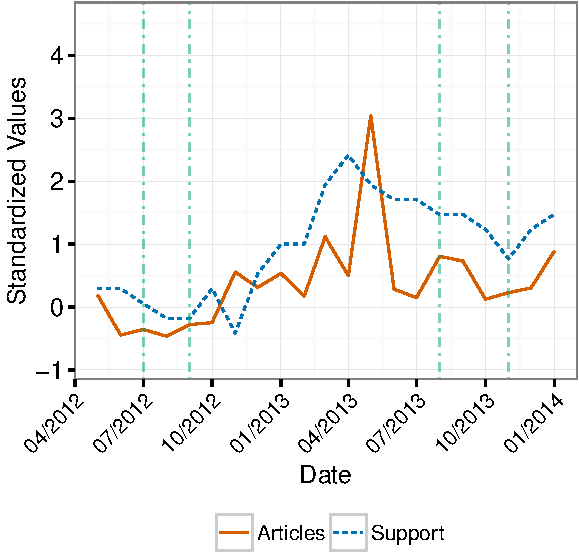
\includegraphics{ukip_media_files/figure-latex/qual-zoomed-plot-1.pdf}
\caption{Standardized Time-Series with Green Dot-Dash Lines Indicating
Non-Responsively Increasing Media Coverage, May 2012 to January 2014}
\end{figure}


\end{document}  